\chapter{System Overview}

\section{Model Architecture}\label{sec:model_arch}
The inspiration from this work comes from~\cite{hierarchical}.
The authors designed a model architecture that can capture 
\begin{itemize}
    \item The architecture builds on what the authors of~\cite{gru4rec} designed.
    \item The model called GRU4Rec uses a RNN using GRUs to model the session data.
    \item The learning task boils down to learn the typical paths users take through the online-store.
    \item This model is not personalized, since we do not use the information which user generated a specific session.
    \item The idea is to predict which product the users wants to see next and provide him or her with a shortcut.
    \item Now we have a fixed size representation of a session.
    \item Now we could try to learn how sessions evolve over time by adding another RNN on the above layer.
    \item This is done by using the session representation as the input, and therefore the hidden state represents the evolvement of the user.
    \item 
    \item Describe how it captures the session representation
    \item illustration for hierarchical neural network
    \item Describe Model Architecture
    \item Describe different Components of Model Architecture
\item Describe different variants of the model (with/without pf, with/without embeddings)
\end{itemize}
\subsection{Model training}
\section{Product Embedding}
\begin{itemize}
    \item We introducted the model architecture for Meta Prod2Vec in~\todo{Add reference to section about metaprod2vec}
    \item We used the features brand, producttype, and price class.
    \item The price class is computed by determining the quantiles of products in the same product type and categorizing the products into 4 price classes.
    \item We used equal weights for all the metadata.
    \item 
    \item 
    \item Write about the features used, what are the transformations etc.
\end{itemize}

\section{Implementation}

\begin{itemize}
    \item we could make a diagram showing the different components
\item Describe Class Diagram
\item Describe prediction mode/training mode
\item Describe problems that arose during training (extensive resources used for so many products and users)
\end{itemize}
\subsection{API}\label{sec:api}
As described above the model is implemented in Tensorflow\footnote{\url{http://tensorflow.org}}.
Tensorflow provides a mechanism to export tensorflow models as so called SavedModel\footnote{\url{https://github.com/tensorflow/tensorflow/blob/master/tensorflow/python/saved_model/README.md}}, which is the way Tensorflow serializes models universally.
They also provide a premade Docker image\footnote{\url{https://hub.docker.com/r/tensorflow/serving}} which allows the model to be served as a REST or GRPC API.
\begin{itemize}
\item Describe API
\end{itemize}

\section{Production Setup}
Digitec Galaxus AG is the largest online-retailer in Switzerland.
They operate galaxus.ch and digitec.ch. The former is a general online-shop comparable to Amazon. 
The latter is specialized in Electronics.
Distributed on the different sections of the site there are several recommendation engines populating the content the users see.
Examples are the landing page\todo{Add screenshot} and multiple engines on the product detail page\todo{Add screenshot}.
% At the time of writing these engines were either recommending products or marketing pages. 
% \par
% Marketing Pages are a part of Digitec Galaxus' marketing strategy.
% There is a editorial team which is separated by a chinese wall from the product departement.
% This team writes independant reviews and other stories including current news.
% These pages give the customers a second reason to interact with the platform, by establishing themselves as a news platform for users.
% Therefore it makes sense to invest in recommendations of articles, since this allows the user to be familiar with the platform, and later preferring it for an online purchase.
% These pages are not considered in this work, however the model should be applicable to marketing pages as well. 

% \subsection{Survival of the Fittest Framework}
% As mentioned above there are multiple locations, such as the product detail page, in which recommendation engines can display content.
% Moreover in each of these locations is it possible to have multiple spots which display content from recommendation engines.
% For example on the product detail page there are multple spots displaying recommendations.
% The Survival of the Fittest Framework is a system designed to decide which recommendation engine runs in which spot. \todo{Show an illustration for the framework}
% The framework is a way of tackling the exploration exploitation tradeoff.
% The definition which recommendation engine is allowed to be displayed in which spot is done manually, since not all combinations of the two make sense from a user experience perspective.
% In principle popular recommendation engines get a proportionally higher probability to be selected when such a page is accessed by a specific user, while maintaining some restrictions.
% This probability of being selected is defined as follows:\todo{Add specific formula}
% \[
%     p_{xij} = max(0.05, )
% \]
% Where $p_{xij}$ is the probability of recommendation engine $x$ being displayed on location $i$ and spot $j$.
% This probability is computed constantly, automatically based on a stream of user clicks.
% The Click-Through-Rate is the relevant metric for this computation because as described in~\ref{conversion_rate} this can only be estimated from the sales, since the true intent of the user cannot be reliably identified.
% Therefore less popular or new recommendation engines still can be selected to be displayed, allowing for exploration of different approaches.
% Should an engine become popular due to an improvement in the logic behind it, the probability of display increases automatically as more users interact with this element.

There is a framework that computes probabilities which specific recommendation engine provides the content for a specific location.
Further the framework then chooses the content for each location based on the probabilities computed before and some other constraints such as minimum and maximum value.
However to test the model implemented in this work this framework is bypassed by a A/B Testing engine, therefore this framework is not part of this work.
The specific tests and the test setup is described in~\ref{sec:exp_setup}, for the understanding of the following it is enough to assume that some independant system is providing recommendation requests to the recommendation system.
Using the API containers described in~\ref{sec:api} we can serve these requests.
The sequence-diagram in figure~\ref{fig:serving_recs} should give an overview on how the system is integrated in the production environment.

\begin{figure}[H]
	\centering
	\captionsetup{width=0.8\textwidth}
    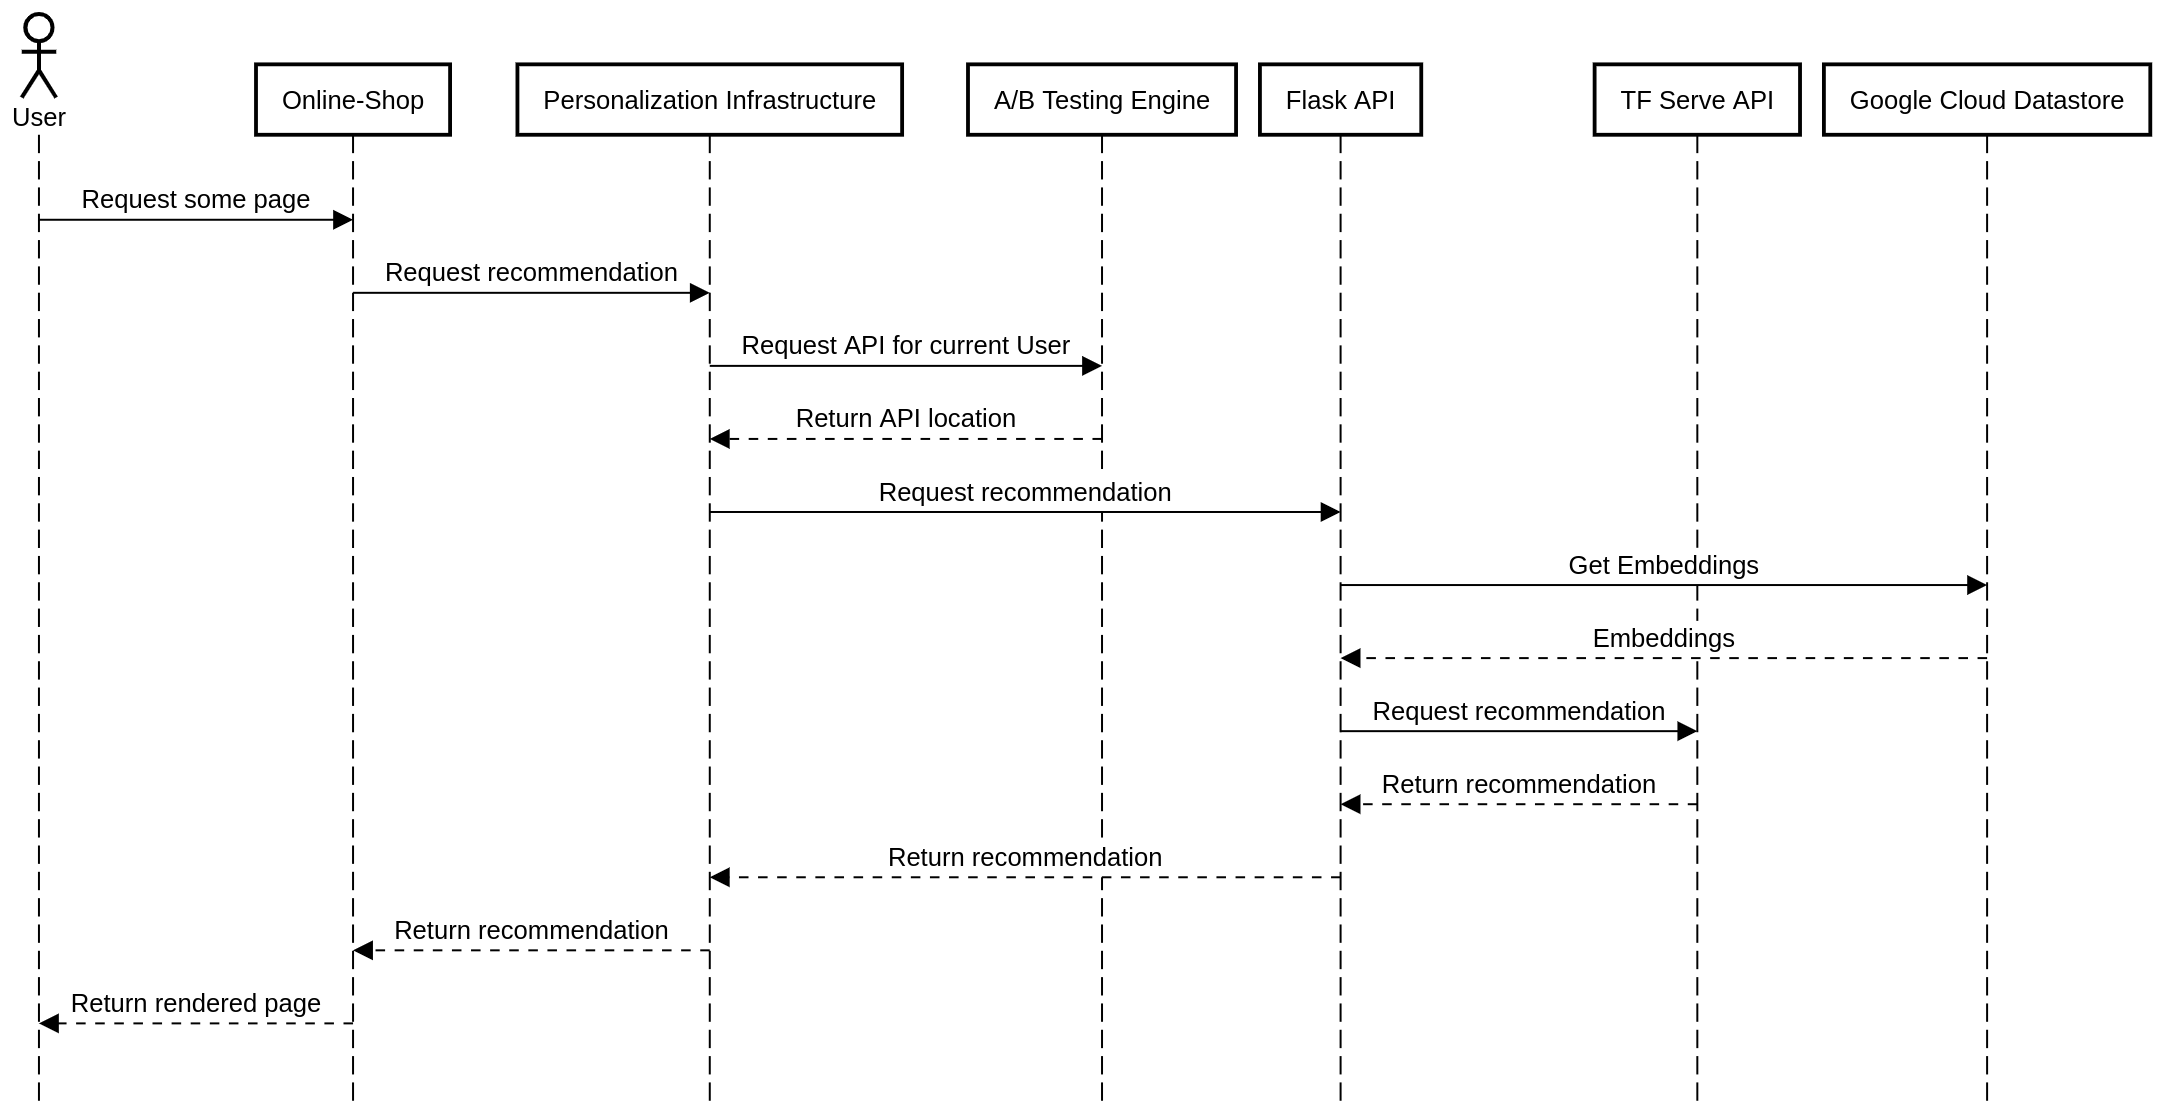
\includegraphics[width=\textwidth]{serving-recommendations.png}
    \caption{Serving Recommendations on digitec.ch and galaxus.ch}
    \label{fig:serving_recs}
\end{figure}

The whole process starts when a specific user requests a specific page on either digitec.ch or galaxus.ch.
If the requested page has an element where there is an A/B test configured the Online-Shop Application will make a request to the testing engine.
As mentioned above the testing engine will then make a request to a API location, which corresponds to one of the model versions.
After that the Online Shop will request the content, in this case, from the Personalization Infrastructure.
Note that during this setup each of the four versions of the model is deployed simultaneously, all of them trained on the same dataset.
The Personalization Infrastructure then calls the API described above.
Before requesting a prediction from tf-serve the API will gather precomputed embeddings for the involved entities.
The predictions are returned to the Personalization Infrastructure and from there to the Online Shop.
The last step is for the Online Shop to render the content and deliver the page to the user.
This process takes about XXms\todo{Get ms number here}ms.